\documentclass[tikz,border=3pt]{standalone}
\usepackage[utf8]{inputenc}
\usepackage[T1]{fontenc}
\usepackage{libertinus}
\usepackage{amsmath,amssymb}
\usetikzlibrary{arrows.meta,calc,patterns,decorations.pathmorphing,decorations.markings,decorations.pathreplacing,bending}
\definecolor{UGblue}{RGB}{0,51,102}
\newcommand{\dbar}{\mathchar'26\mkern-12mu d}
\tikzset{
  >=Stealth,
  every node/.style={font=\small},
  caja/.style={draw,line width=0.9pt},
  pared/.style={draw,line width=1.6pt},
  ejes/.style={->,line width=0.8pt},
  adia/.style={draw,pattern=north east lines,pattern color=black!70,line width=0.5pt},
  gas/.style={fill=UGblue!8},
  punto/.style={fill,circle,inner sep=1.3pt},
  onda/.style={decorate,decoration={snake,amplitude=1.1pt,segment length=5pt,post length=3pt,pre length=0pt}},
}
\begin{document}
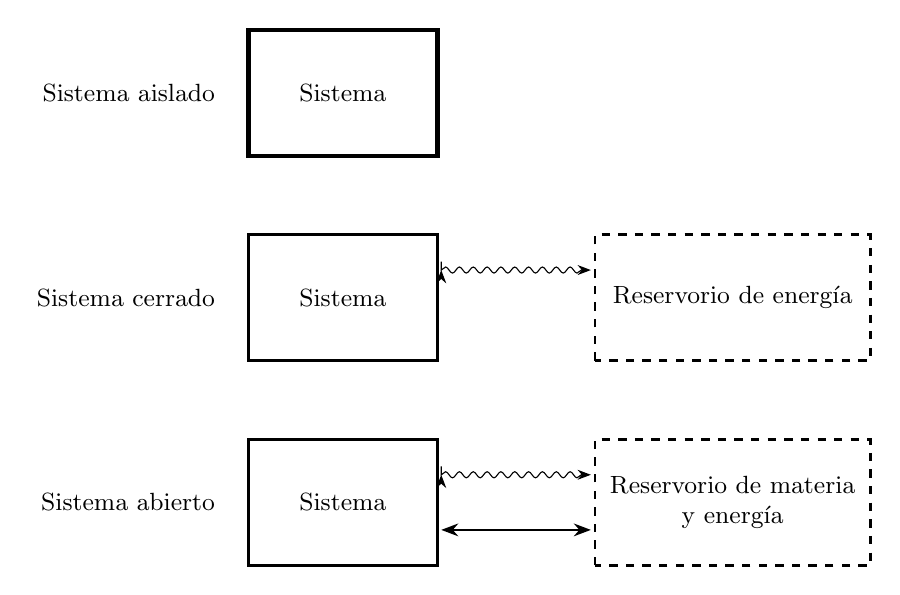
\begin{tikzpicture}
  \node[anchor=east] at (-0.3,0.8) {Sistema aislado};
  \draw[caja] (0,0) rectangle (2.4,1.6) node[midway] {Sistema};
  \draw[pared] (0,0) rectangle (2.4,1.6);
  \node[anchor=east] at (-0.3,-1.8) {Sistema cerrado};
  \draw[caja] (0,-2.6) rectangle (2.4,-1.0) node[midway] {Sistema};
  \draw[caja,dashed] (4.4,-2.6) rectangle (7.9,-1.0);
  \node[align=center] at (6.15,-1.8) {Reservorio de energía};
  \draw[onda,<->] (2.45,-1.4500000000000002) -- (4.35,-1.4500000000000002);
  \node[anchor=east] at (-0.3,-4.4) {Sistema abierto};
  \draw[caja] (0,-5.2) rectangle (2.4,-3.6) node[midway] {Sistema};
  \draw[caja,dashed] (4.4,-5.2) rectangle (7.9,-3.6);
  \node[align=center] at (6.15,-4.4) {Reservorio de materia\\y energía};
  \draw[onda,<->] (2.45,-4.050000000000001) -- (4.35,-4.050000000000001);
  \draw[<->,line width=0.7pt] (2.45,-4.75) -- (4.35,-4.75);
\end{tikzpicture}
\end{document}
